\documentclass[tikz,border=10pt]{standalone}
% No TikZ libraries needed for plain segments and labels.
\begin{document}
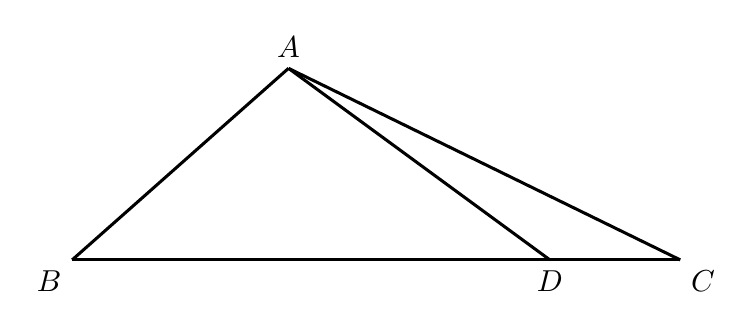
\begin{tikzpicture}[line join=round, line width=1.1pt]
  % Vertices: pixel -> units with s = 0.009357, centred on ink bbox (cx=464, cy=205)
  \coordinate (A) at (-1.1204, 1.2164);
  \coordinate (B) at (-3.8683, -1.2164);
  \coordinate (C) at (3.8551, -1.2164);
  \coordinate (D) at (2.1996, -1.2164);

  % Triangle sides and cevian AD (all solid)
  \draw (A) -- (B);
  \draw (B) -- (C);
  \draw (C) -- (A);
  \draw (A) -- (D);

  % Vertex labels (math mode, 10.5pt font per cap-height metrics)
  \node[font=\fontsize{10.5}{12.6}\selectfont, above] at (A) {$A$};
  \node[font=\fontsize{10.5}{12.6}\selectfont, below left] at (B) {$B$};
  \node[font=\fontsize{10.5}{12.6}\selectfont, below right] at (C) {$C$};
  \node[font=\fontsize{10.5}{12.6}\selectfont, below] at (D) {$D$};
\end{tikzpicture}
\end{document}